\documentclass{article}

\usepackage{lipsum}
\usepackage[margin=1in,includefoot]{geometry}
\usepackage{graphicx}
\usepackage{float}
\usepackage[hidelinks]{hyperref}
\usepackage{amsmath}
\usepackage{lscape}
\usepackage{enumitem}

\usepackage[english]{babel}
\usepackage[utf8x]{inputenc}
\usepackage{multirow}
\usepackage{float}
\usepackage{multirow}
\usepackage[superscript,biblabel]{cite}




% Header and Footer Stuff
\usepackage{fancyhdr}
\pagestyle{fancy}
\fancyhead{}
\fancyfoot{}
\fancyfoot[R]{\thepage}
\renewcommand{\headrulewidth}{0pt}
\renewcommand{\footrulewidth}{0pt}

\begin{document}



\thispagestyle{empty}
\cleardoublepage
\pagenumbering{arabic}
\setcounter{page}{1}


\section{COMING UP WITH AN IDEA - Brainstorming report }\label{sec:intro}



The ideas resulting of the brainstorming session are:
	
\begin{enumerate}
	\item Refugee  Detection System: An aerial system which through high def cameras is stationed in a large body of water. The cameras will use infrared tech and deep learning algorithm to predict and detect refugee boats in the mediterranean sea.

	\item Hands Free Medical Tablet: In order to avoid cross infection in hospitals due to the contact of professionals on screens, one tablet led by the eyes can help.

	\item Exosuits for disabled 

	\item DNA Computer: Knowing that DNA is a very condensed storage of information in our body, the intention was to apply this to the new technologies by using a nucleobases code instead of a binary one. 

	\item Change of currency: Machine which converts the money of one currency to another.

	\item Global/Remote Internet services: Using self-sustainable light aircraft to provide internet connectivity in extremely remote areas of the world.

	\item Household utility Computer with Operating System: A lot of daily household activities now have the ability to be automated. This computer would integrate all the functionalities into one UI and make it configurable via smartphone or voice activation. 

	\item\underline{Virtual Reality for surgery assist}
\end{enumerate}
The optics and image techniques in the surgery field have a very important role. Before a surgery, structural or functional images are required in order to focalise where the pathogenic mechanism is occurring. They are more important still in the case of laparoscopy and endoscopy, in which they are the eyes of the surgeon. However, the surgeon must divert attention to look at the screen to see this information or to be able to follow the surgery. For this reason, a head display will be useful and also can act as diagnosis tool in real time. The head-up display will be based on a number of principal.

The heads up display seeks to constantly update the surgeon on the patient's vitals as to minimize fatigue and make it more comfortable for the surgeon to operate.
Secondly, using a sensitive camera sensor, the patient's vital blood vessels can also be detected, mapped, and displayed in the augmented-reality display system. This is to alarm  the surgeon of possible dangers in a given situation of operation, such as cutting below that tissue, or to show the surgeon where and how deep that vessel is.
Thirdly the system would function as a recording system for hospitals, hopefully reducing the insurance cost of hospitals and the amount of legal difficulties associated with an unsatisfactory end to a surgery, or forgotten equipment within a patient, which has previously happened in various cases.
Finally, the display would serve as a guide and teaching apparatus for new surgeons to see how a surgery is operator or for experienced surgeons to examine past surgeries and improve on the standard of care given, thus allowing future surgeons to learn on a much more intimate level of knowledge, as the perspective of the viewing is different from simply that of an onlooker.
\begin{align*}
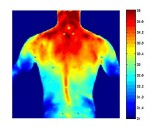
\includegraphics[height =4cm]{pic1.jpg}
\quad

\includegraphics[height=4cm]{pic2.jpg}
\end{align*}
\end{document}